\documentclass[tikz,border=4pt]{standalone}
\usepackage{amsmath}
\begin{document}
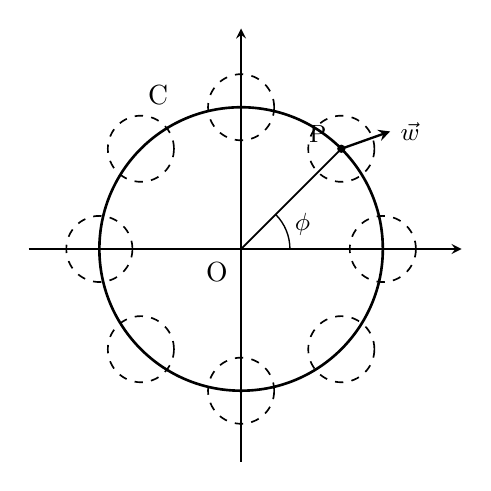
\begin{tikzpicture}[>=stealth, thick, scale=1.0]
  % Coordinate axes
  \draw[->, line width=0.6pt] (-2.7, 0) -- (2.8, 0);
  \draw[->, line width=0.6pt] (0, -2.7) -- (0, 2.8);
  \node[below left] at (-0.04, -0.04) {$\mathrm{O}$};

  % Unit circle C (radius R = 1.8)
  \draw[line width=0.95pt] (0, 0) circle (1.8);
  \node[above left] at (115:1.88) {$\mathrm{C}$};

  % Eight dashed small circles centered at angles 0, 45, ..., 315 deg
  \foreach \ang in {0, 45, 90, 135, 180, 225, 270, 315} {
    \draw[dashed, line width=0.6pt] (\ang:1.8) circle (0.42);
  }

  % Radius vector to P at 45 deg and vector w from P
  \coordinate (P) at (45:1.8);
  \draw[line width=0.65pt] (0, 0) -- (P);
  \fill (P) circle (1.5pt);
  \node[above left, font=\small] at (45:1.72) {$\mathrm{P}$};

  % Angle phi
  \draw[line width=0.5pt] (0.62, 0) arc[start angle=0, end angle=45, radius=0.62];
  \node[font=\small] at (22:0.84) {$\phi$};

  % Arbitrary vector w originating at P
  \draw[->, line width=0.85pt] (P) -- ++(0.62, 0.22) node[right, font=\small] {$\vec{w}$};
\end{tikzpicture}
\end{document}
